\section{Gaussian Process Model}\label{sec:gpmodel}
A GP can be applied as a probabilistic model to a regression problem.  Here we use the GP model to generalise a stellar model grid to a continuous and probabilistic function that maps inputs to observable quantities.  This will allow us to predict observable quantities that are off the grid of stellar models with the prediction including uncertainty. 
%
We intend to train GP models that maps five fundamental inputs,  i.e., mass ($M$), initial metallicity ([Fe/H]$_{\rm init}$), initial helium fraction($Y_{\rm init}$), the mixing-length parameter($\alpha_{\rm MLT}$), and equivalent evolutionary phase ({\it EEP}), to five model outputs including effective temperature($T_{\rm eff}$), surface gravity($\log g$), radius($R$), surface metallicity({\it [Fe/H]}), and stellar age($\tau$). We use the GP model as a non-parametric emulator, that is emulating the comparatively slow calls to models of stellar evolution.
This emulator can be described as a function approximation problem. In fact, the way we have implemented the GP as function approximation means that we have used one GP for each of the outputs so that they can be described as
\begin{equation}\label{gprmodel1}
{T_{\rm eff}} = f_{T_{\rm eff}}(M, EEP, ({\rm Fe/H})_{\rm init}, Y_{\rm init}, \alpha_{\rm MLT}),
\end{equation}
\begin{equation}\label{gprmodel1}
{\log g} = f_{\log g}(M, EEP, ({\rm Fe/H})_{\rm init}, Y_{\rm init}, \alpha_{\rm MLT}),
\end{equation}
\begin{equation}\label{gprmodel1}
{R} = f_{R}(M, EEP, ({\rm Fe/H})_{\rm init}, Y_{\rm init}, \alpha_{\rm MLT}),
\end{equation}
\begin{equation}\label{gprmodel1}
{[Fe/H]} = f_{[Fe/H]}(M, EEP, ({\rm Fe/H})_{\rm init}, Y_{\rm init}, \alpha_{\rm MLT}),
\end{equation}
and 
\begin{equation}\label{gprmodel1}
{\tau} = f_{\tau}(M, EEP, ({\rm Fe/H})_{\rm init}, Y_{\rm init}, \alpha_{\rm MLT}).
\end{equation}
In the following, we introduce the underline theory of GP regression and the setup of training GP models.  


\subsection{Gaussian Process Application}

In our application to a stellar model grid, a GP has a number of desirable properties. While a GP is a stochastic process, the distribution of a GP can be considered as a distribution of functions with a continuous domain.  In fact,  the marginal likelihood considered in function space is equal to the likelihood of the data given some function values,  multiplied by the prior on those function values marginalised over all function values \cite{williams1996gaussian}.  That is to say that, the GP allows for the analytical evaluation of a fit over many different functions (perhaps an infinite number) weighted by some concept of a prior and the agreement with the data. In addition, while the marginal likelihood will be assessed on discrete data,  predictions can be made using linear algebra for new data in the continuous domain, but crucially again marginalised over these many different functional forms.  It is possible to see how this might be useful for generalising (or emulating or augmenting) a discrete grid of stellar models in order to obtain predictions in the continuous domain.

In this section we will look at the required mathematics to be able to implement a GP for our application to grids of stellar models.  We start with a series of definitions before dealing with the marginal likelihood and the posterior predictive distributions. 

We start with a grid of stellar models containing $N$ models with a label we want to learn, for example model effective temperature, which we will denote with the general symbol $\bf y$, and a set of on-grid inputs $\bf X$ (e.g., mass,  {\it EEP},  metallicity,  ...).  We can use a GP to make predictions of the effective temperature (labelled $y$) for additional off-grid input values given by $\bf X_{\star}$.  The vector $\bf y$ is arranged ${\bf y} = \left(y_{i}, ... ,y_{N} \right)^{T}$ where the subscript label references the stellar model.  The input labels are arranged into a $N \times D$ matrix where $D$ is the number of input dimensions (e.g., $D=3$ for mass, {\it EEP}, and metallicity) so that ${\bf X} = ({\bf x}_{1}, ..., {\bf x}_{N})^{T}$ where ${\bf x_{i}} = (x_{1, i}, ..., x_{D, i})^{T}$.  The matrix of additional inputs $\bf X_{\star}$ has the same form as $\bf X$ but size $N_{\star} \times D$.

\citet{williams1996gaussian}, from which our description below is based,  define a GP as a collection of random variables, where any finite number of which have a joint Gaussian distribution.  In general terms,  a GP may be written so that our on grid labels are random variables drawn from our GP distribution, 
\begin{equation}
{\bf y}({\bf X}) \sim \mathcal{GP}\left( m({\bf X}),  {\bf \Sigma}\right),
\end{equation}
where $m({\bf X})$ is some mean function, and $\bf \Sigma$ is some covariance matrix.  The mean function controls the deterministic part of the regression and the covariance function controls the stochastic part.  The mean function defined here could be any deterministic function and we will label the additional parameters, or hyperparameters, $\phi$.  Each element of the more familiar covariance matrix is defined by the covariance function or {\it kernel function} $\bf K$ which has hyperparameters $\theta$ and is given by,
\begin{equation}
{\bf \Sigma} = {\bf K}({\bf X}, {\bf X},  \theta),
\end{equation}
or 
\begin{equation}
{\bf \Sigma}_{n, m} = k({\bf X}_{n}, {\bf X}_{m},  \theta),
\end{equation}
where the inputs ${\bf X}_{n}$ and ${\bf X}_{n}$ are $D$-dimensional vectors and the output is a scalar covariance.
In addition to the covariance defined by the kernel function, we include additional white noise in the covariance matrix by adding an identity matrix $\mathcal{I}$ multiplied by a scalar value $\sigma_{w}^2$, so that, 
\begin{equation}
{\bf \Sigma} = {\bf K}({\bf X}, {\bf X},  \theta) + \sigma_{w}^{2} \mathcal{I},
\end{equation}
where $\sigma_{w}^2$ is another hyperparameter to be learnt in training. 

\subsubsection{The likelihood}
Conceptually we value the GP because of it's ability to marginalise over many functions $\bf f$ and return a marginal likelihood,
\begin{equation}
p({\bf y} | {\bf X}) = \int p({\bf y} | {\bf f}, {\bf X}) p({\bf f} | {\bf X}) \, {\rm d}{\bf f},
\end{equation}
noting that this function space marginal likelihood is weighted by the probability of the data given the function and the probability of the function.  This integral could be evaluated.  However, by noting that a GP is a collection of random variables, where any finite number of which have a joint Gaussian distribution, the marginal probability of our data $\bf y$ is also the joint likelihood of a multivariate normal distribution,
\begin{equation}
p({\bf y} | {\bf X}) = \mathcal{N}(m({\bf X}), {\bf \Sigma}),
\end{equation}
which can be straightforward to evaluate. Thus the marginal likelihood is,
\begin{equation}
p({\bf y} | {\bf X}) = (2 \pi)^{k/2} {\rm det} ({\bf \Sigma})^{-0.5} \exp \left(\frac{-1}{2} ({\bf X} - m({\bf X}))^{T} \, {\bf \Sigma}^{-1} \, ({\bf X} - m({\bf X})) \right),
\end{equation}
which can be evaluated without integrating over all possible function space. While this marginal likelihood expression is clearly more computationally feasible that the integral over functional space it not without it's limitations.  Because it is necessary to calculate the determinant and the inverse of the covariance matrix, typically applied algorithms,  make this a $\mathcal{O}(N^3)$ or $\mathcal{O}(N^2 \log N)$ operation.  This naturally limits the size of the data set for which the likelihood,  and optimisations of the likelihood, can be applied.  

\subsubsection{Making predictions}
If we want to obtain predictive distributions for the output $\bf y_{\star}$ given the inputs $\bf X_{\star}$,  the joint probability distribution of $\bf y$ and $\bf y_{\star}$ is Gaussian and given by
\begin{equation}
p \left( \begin{bmatrix} {\bf y} \\ {\bf y_{\star}} \end{bmatrix} \right) = \mathcal{N} \left( \begin{bmatrix} m({\bf X}) \\ m({\bf X_{\star}}) \end{bmatrix} , \begin{bmatrix} {\bf \Sigma} & {\bf K_{\star} }\\ {\bf K_{\star}}^{T} & {\bf K_{\star \star}} \end{bmatrix}  \right), 
\end{equation}
where the covariance matrices $\bf \Sigma$ and $\bf K$ are computed using the kernel function so that,

\begin{equation}
{\bf \Sigma}_{n, m} = k({\bf X}_{n}, \, {\bf X}_{m}),
\end{equation}
which is an $N \times N$ matrix.
\begin{equation}
{\bf K}_{\star \, n, m} = k({\bf X}_{n}, \, { \bf X}_{\star \, m}),
\end{equation}
which is an $N \times N_{\star}$ matrix, and finally
\begin{equation}
{\bf K}_{\star \star \, n, m} = k({\bf X}_{\star \, n},  {\bf X}_{\star \,m}),
\end{equation}
which is an $N_{\star} \times N_{\star}$ matrix.
The predictions of $\bf y_{\star}$ are again a Gaussian distribution so that,
\begin{equation}
{\bf y}_{\star} \sim \mathcal{N}(\bf \hat{y}_{\star}, \, \bf C),
\label{eq:pred}
\end{equation}
where 
\begin{equation}
{\bf \hat{y}}_{\star} = m({\bf X}_{\star}) + {\bf K}_{\star}^{T} \, {\bf \Sigma}^{-1} \, ({\bf y} - m(\bf X)),
\end{equation}
and 
\begin{equation}
{\bf C} = {\bf K}_{\star \star} - {\bf K}_{\star}^{T} \, {\bf \Sigma}^{-1} \, {\bf K_{\star}}.
\end{equation}

At point we can make predictions on model properties given a grid of stellar models using equation \ref{eq:pred}.  But these predictions will likely be poor unless we select sensible values for the form and hyperparameters of the mean function and covariance function.  In the following section we detail a number of kernel functions that will be tested against the data.  We will then discuss the method for determining the values of the hyperparameters to be used.


\subsection{Setup of GP Models}\label{sec:setup}

\subsubsection{Tool package}

We adopt a tool package named \textsc{GPyTorch}, which is a GP framework developed by \citet{gardner2018gpytorch}. It is a Gaussian process library based on an open source machine-learning framework PyTorch (\url{https://pytorch.org}). The package provides significant GPU acceleration, state-of-the-art implementations of the latest algorithmic advances for scalability and flexibility, and easy integration with deep learning frameworks. Source codes and detailed introductions could be found on \url{https://gpytorch.ai}. 
%
All the trainings are on an NVidia Tesla V100 graphics processing unit (GPU) with 32GB GPU Memory. The GPU captivity allows training up to $\sim$20,000 data points for a GP model. 


\subsubsection{Training procudure}

The training procedure of a GP model includes training, validating, and testing. 
In the training process, we literately optimise hyperparameters of a GP model to learn the underline function which maps inputs to outputs from on-grid evolutionary tracks (training dataset). In each iteration, the GP model is validated by comparing true and GP predicted values of off-grid tracks (validating dataset). Although the validating dataset is not directly involved in training hyperparameters, it still constructs the GP model to some extend because the optimal solution is the one that best fits the validating dataset. For this reason, the validating dataset does not give a completely independent validation for a GP model. We hence have a testing process at the end. We do this by reserving a half of off-grid tracks from the training and validating process. These tracks (testing dataset) are used to estimate the systematic errors/uncertaintues of GP model. 

Here we briefly summary the setup of GP model training. We apply an architecture Neural Network including 6 hidden layers and 128 nodes per layer as the mean function. The \textsc{Gpytorch} standard likelihood for regression, which assumes a standard homoskedastic noise model, is used as the likelihood function, and we the negative logarithm of the likelihood as the loss function. The optimiser for training is called `Adam', whic is a combination of the advantages of two other extensions of stochastic gradient descent, specifically, Adaptive Gradient Algorithm and Root Mean Square Propagation. 
%
To avoid overfitting, we set up an Early Stopping by monitoring the validating errors. The training is terminated when there is no improvement in validation error for 300 iterations. The GP model is saved when the so-far best validation result is found. Detailed discussions about these setup can be seen in the Appendix \ref{app:A}. 

\subsubsection{Kernel Function}\label{sec:kernel}

To select the proper kernel function for training GP models, we test four basic kernels and a number of combined kernels. 
%
The four basic kernels are listed as follow. 
\begin{itemize}
\item {\bf RBF}: Radial Basis Function kernel (also known as squared exponential kernel)
\item {\bf RQ}: Rational Quadratic Kernel (equivalent to adding together many RBF kernels with different lengthscales)
\item {\bf Mat12}: Matern 1/2 kernel (equivalent to the Exponential Kernel)
\item {\bf Mat32}: Matern 3/2 kernel 
\end{itemize}
These four kernels are all universal, and we can integrate each of them against most functions. Every function in its prior has infinitely many derivatives. The differences between these kernels can be simply understood as their different smoothness and complexity. The RBF kernel is very smooth and suits for the case when the data follow a slowly varying function. The RQ kernel, as a combination of many RBF kernels, is more complex and is able to fit to data with a number of smooth underline functions (e.g. when the output depends on some inputs in different ways). One the opposite, the Mat12 kernel is very spiky and it can fit any sharp variations in the data. The Mat32 kernel has a smoothness somewhere between the RBF and Mat12 kernels. It is a smooth function but has significantly more extrema than the RBF kernel. 
%
These differences are not chance coincidence, and the origin of these differences are crucial for interpreting the results. Choosing a good kernel for a particular application is necessary for good predictions. If the generates functions that are too spiky, then the analysis will have variance that is too high. On the contrary, if the kernel function is too smooth, it may not fully capture the variability of the underlying function and lead to an increase in bias.
%
Combining basic kernels can increase the complexity or flexibility of kernel function. For instance, the combination of a RBF kernel and a Mat12 kernel is able to fit to both smooth and spiky features in the data. However, the risk of using combined kernel (increasing the complexity or flexibility of kernel function) is overfitting. 

According to the stellar theory, changing fundamental input parameters smoothly changes the dependent outputs. Hence the kernel function for our application needs to be smooth. Moreover, we can notice in Figure \ref{fig:eep} that the observable quantities fast vary at some particular regions (e.g., around the `hook'). This means that a slowly varying function like the RBF kernel may under fit in these areas. We do a number of preliminary studies of training GP models with different kernel functions to choose the proper kernel function. Details of training will be mentioned in Section \ref{sec:2d}. Here we only summary the results. 
%
We apply four basic kernels and a number of their combinations (RBF + Mat21, RQ + Mat21, Mat32 + Mat21, RBF + Mat32, RQ + Mat32) to train GP models, and then test GP predictions with off-grid models which are not involved in the training. The combined kernel RBF+Mat21 gives the best fit to the training data, however, its testing errors are large. This indicates that the kernel is too flexible and hence overfits to the data.  
%
The kernel having the best performance is the Mat32. The GP model with Mat32 fits training data reasonably well and gives the best predictions for the testing models. 
%
The results match our expectations. What we need is a smooth function but not too smooth to fit to the quick variations at some particular evolutionary phases. The Mat32 kernel is apparently suitable for our application. 

\section{Preliminary Studies}\label{examples}

Before training the whole model grid (with five input demissions), we start with a number of preliminary studies on low-demission dataset. 
%
These preliminary studies are for several purposes. In the 1D problem (training data on a single evolutionary track), we compare GP predictions with the classical interloper using the quadratic function. In the 2D problem, we train GP models on a mass -- {\it EEP} platform to test the performances of using different kernel functions. We also discuss about introducing a new error index to validating and testing GP models instead of using a global error quantity such like Root Mean Square Error.
%
In the 3D problem, where GP maps three fundamental inputs (mass, EEP, and metallicity) to observables, we solve the training strategy for large dataset whose data size excesses the practical limitation of a GP model. 

\subsection{1D Problem}

We first demonstrate an example of GP application on an 1D problem. We train a GP model using the Mat32 kernel to learn the evolution of effective temperature for a $\rm 1.1M_{\odot}$ track. 
%
We split the model data points on this track into training and testing data by 70-to-30. We train a GP model which maps  {\it EEP} to effective temperatures and then compare GP-predicted effective temperatures with truths. As it can be seen in Figure \ref{fig:1dgp}, the GP model gives very good predictions with all residuals less than $\pm$0.5 K. As a comparison, we fit the training data with the quadratic function and use it to do the same predictions. As it shown that we find very similar results from the two methods. It suggests that GP can be an alternative of classical interpolators on the 1D problem. 

\begin{figure}
	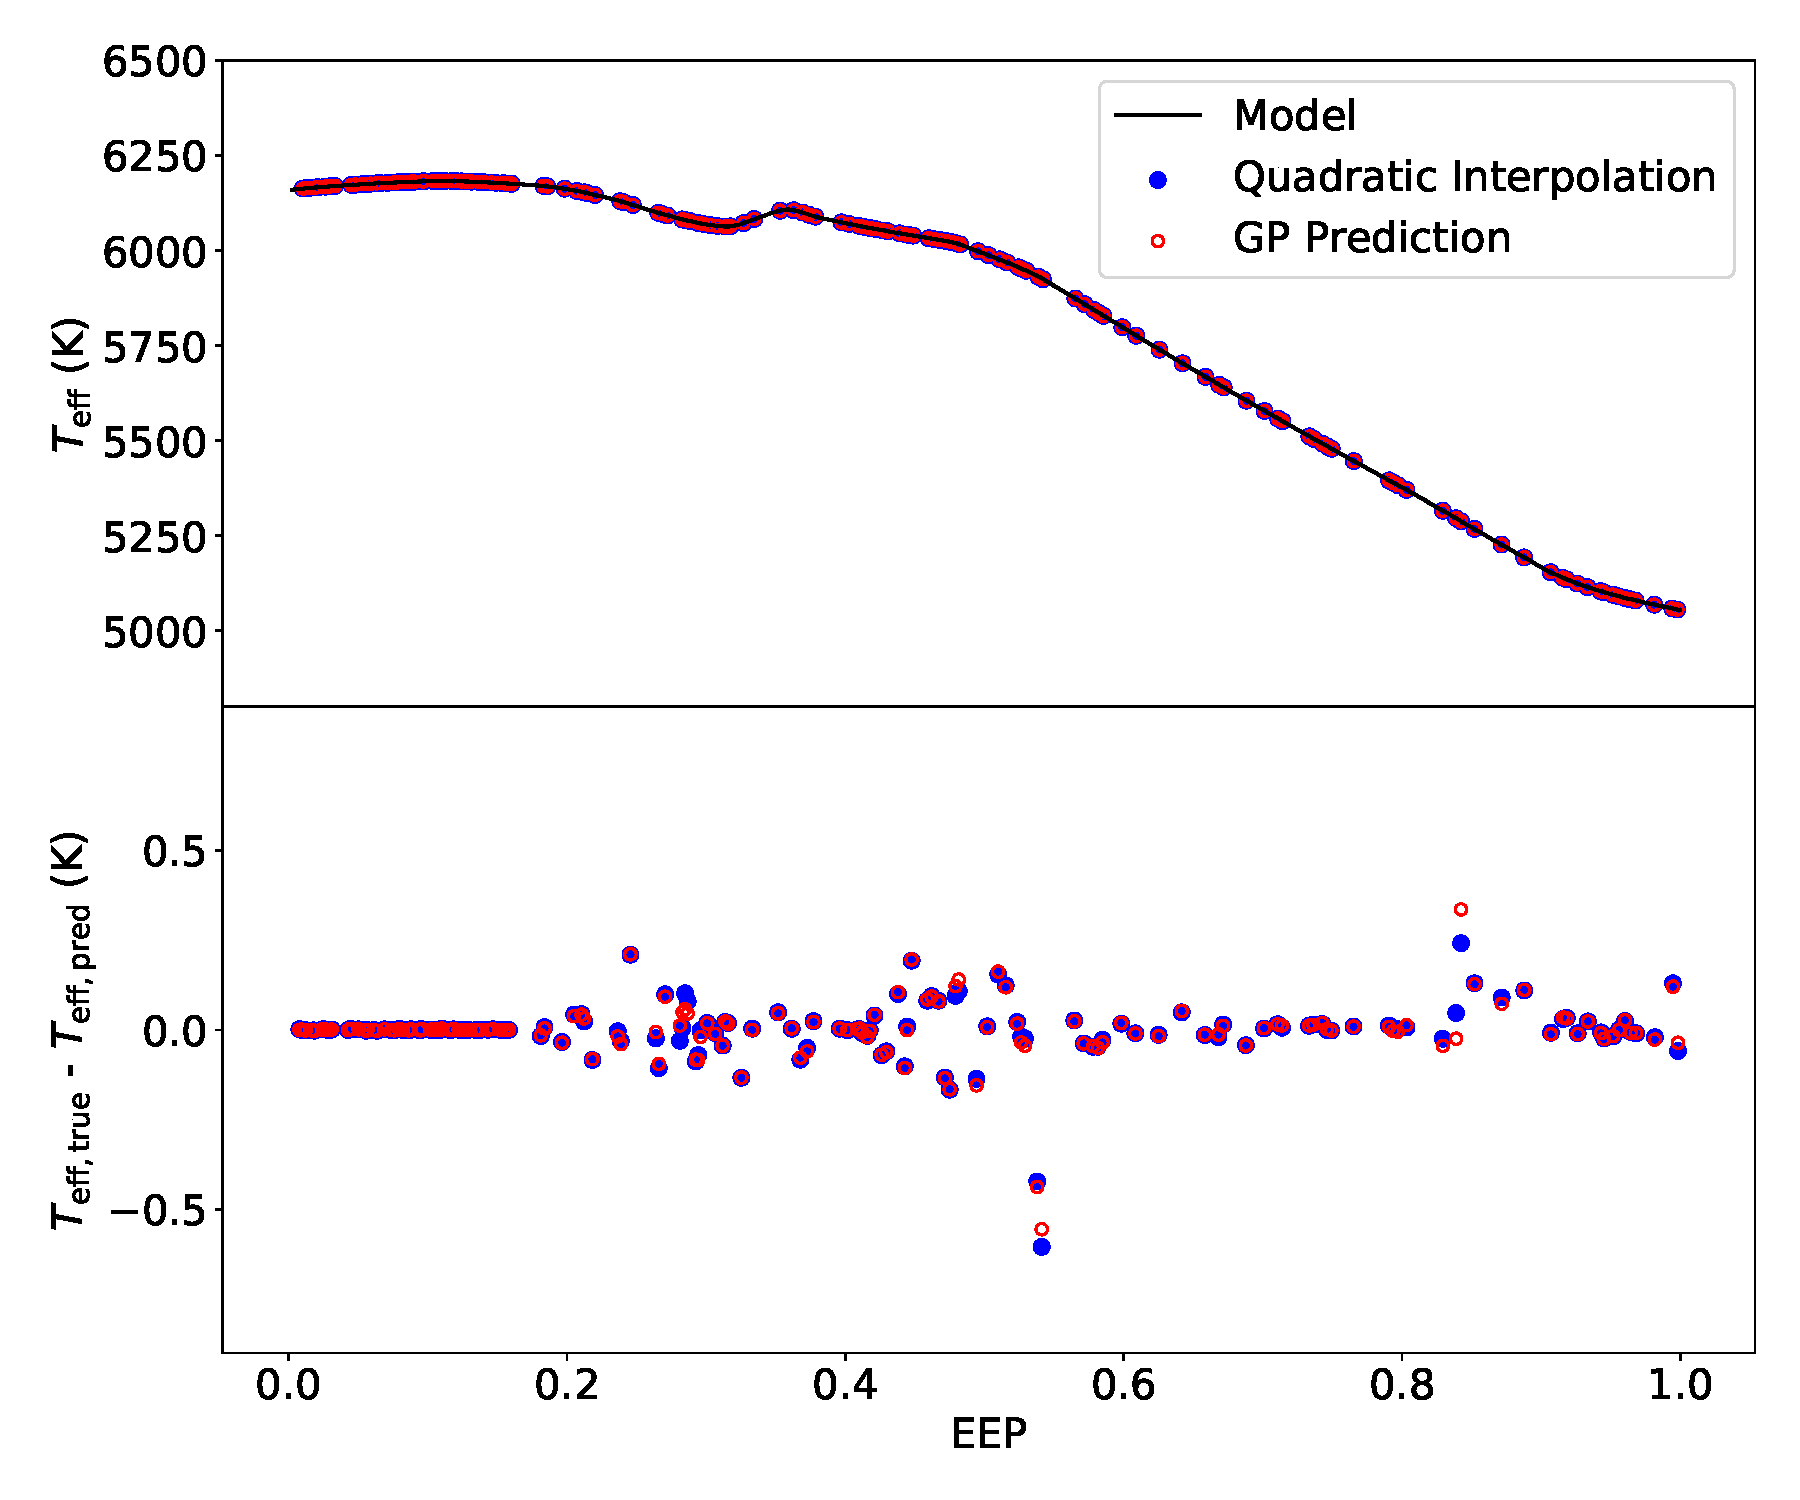
\includegraphics[width=1.0\columnwidth]{1d-gp.pdf}
    \caption{GP application on 1D problem. Models on this track are split into training and testing data by 70-to-30, Top: the evolution of effective temperature for a $\rm 1.1M_{\odot}$ track. The grey line is the evolutionary track computed with \textsc{MESA}; blue and red circles indicate predictions for the testing data from the quadratic interpolator and the GP model. Bottom: residuals of predictions in the top graph. }  
    \label{fig:1dgp}
\end{figure}

\subsection{2D Problem}\label{sec:2d}

As a further step, we train GP models for the 2D problem where GP models map mass and {\it EEP} to the five observable outputs (Outputs = $f(M, EEP)$). Training data are selected from the primary grid with fixed [Fe/H]$_{\rm init}$ (0.0), $Y_{\rm init}$ (0.28), and $\alpha_{\rm MLT}$ (2.1). There are 41 evolutionary tracks which content 24,257 models, and we sample 20,000 of them. To validate and test GP models, we compute 44 evolutionary tracks with the same [Fe/H]$_{\rm init}$, $Y_{\rm init}$, and $\alpha_{\rm MLT}$ but random $M$. We split the off-grid track half-to-half as validating and testing datasets. 
%
Our code for training is developed based on the \textsc{Simple GP Regression} example (\url{https://docs.gpytorch.ai/en/stable/examples/01_Exact_GPs/Simple_GP_Regression.html}). We change the mean function and optimiser in the example and add an early stopping and a model saving modules. The script used for the training this 2D problem can be seen at \url{somewhere-at-github}. 
%
We follow the aforementioned training procedure to train, validate, and test GP models. We illustrate the GP model (with the Mat32 kernel) for effective temperature on the mass--{\it EEP} diagram in Figure \ref{fig:2dtest}. As it shown that, GP transforms the sparse data into a continuous function and hence is able to predict values for unseen points in the grid. 
%

\begin{figure}
	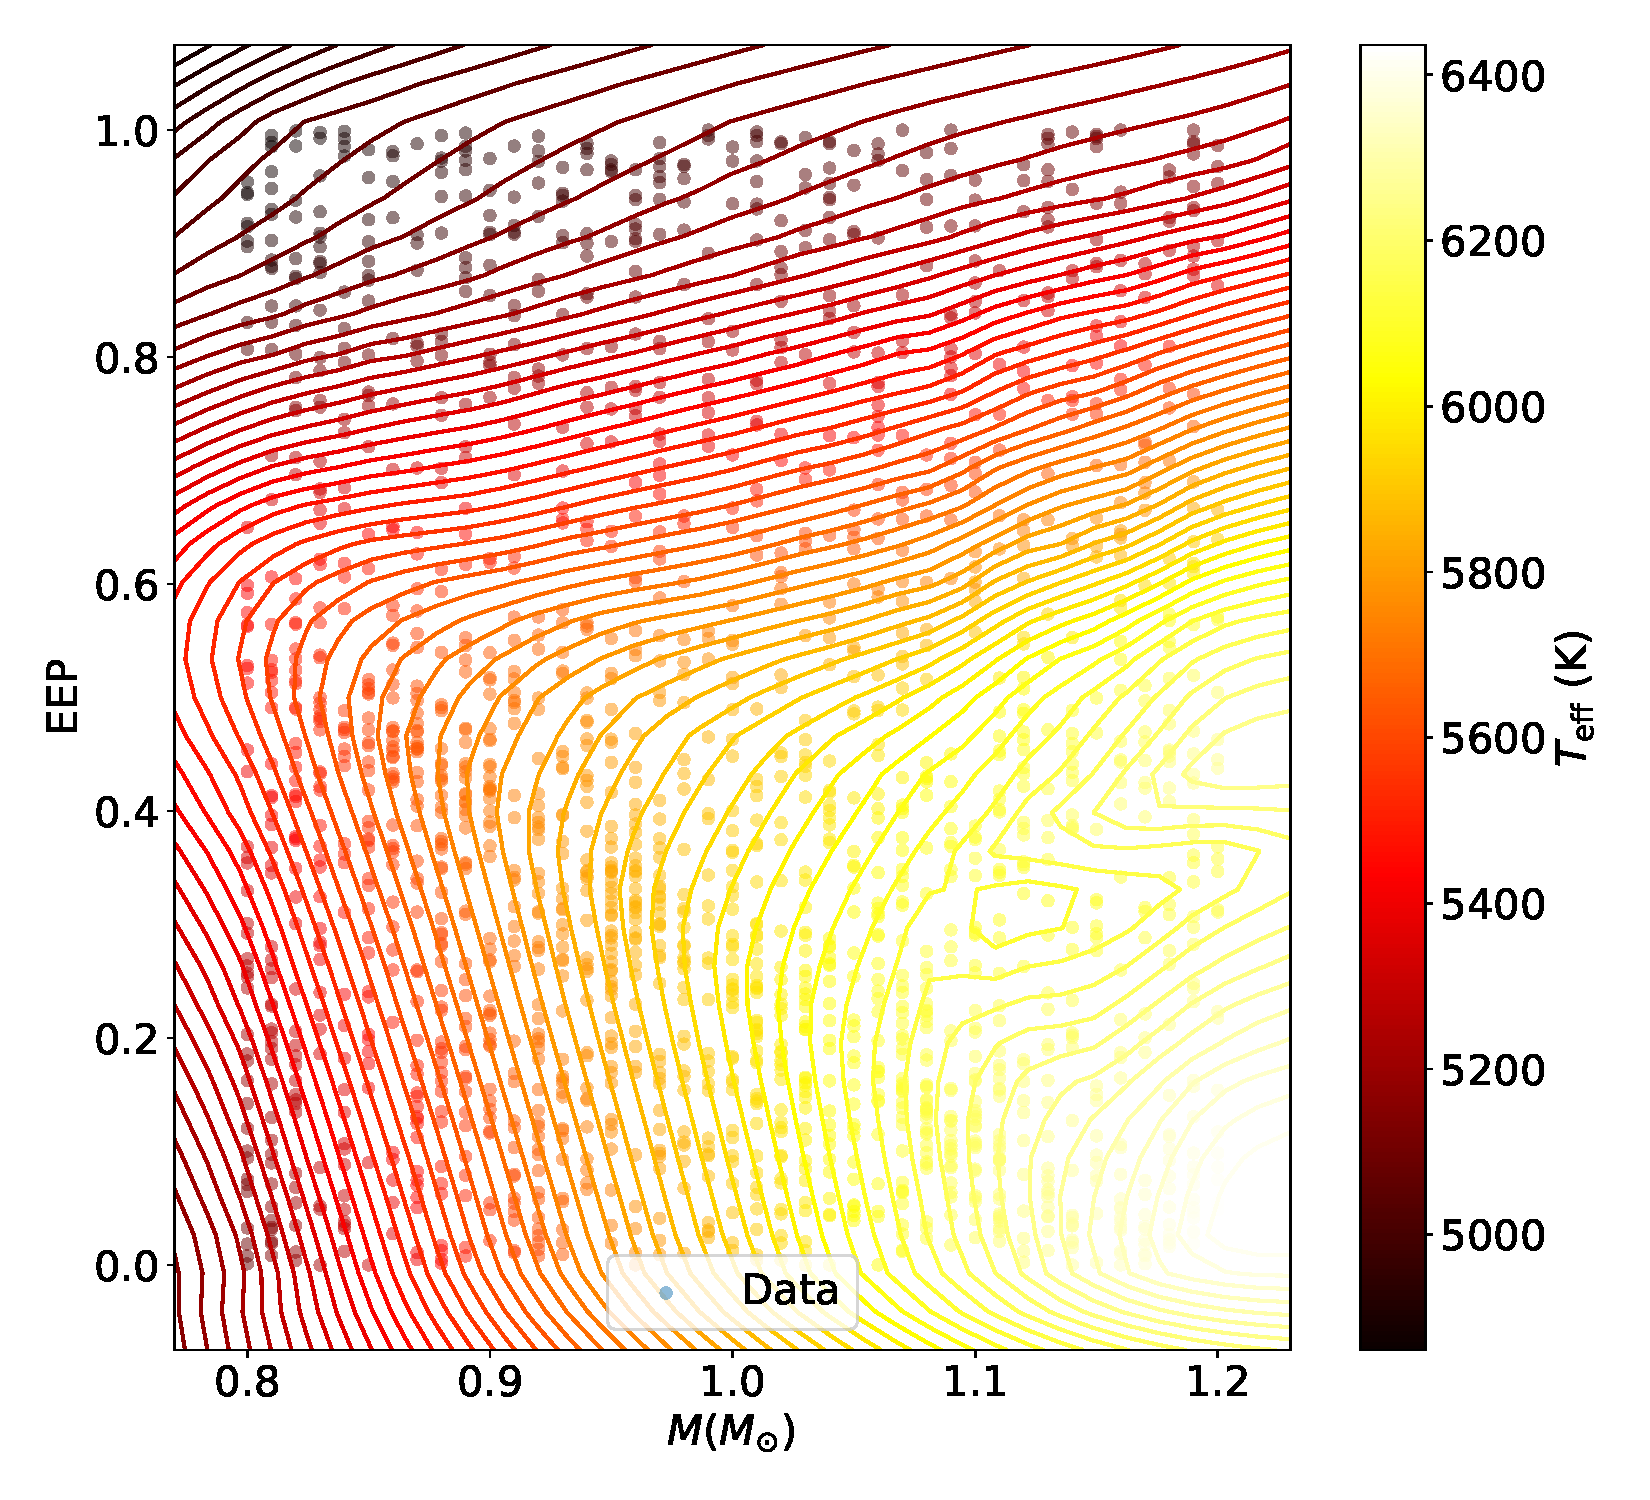
\includegraphics[width=1.0\columnwidth]{2d_GPmodel_function.pdf}
	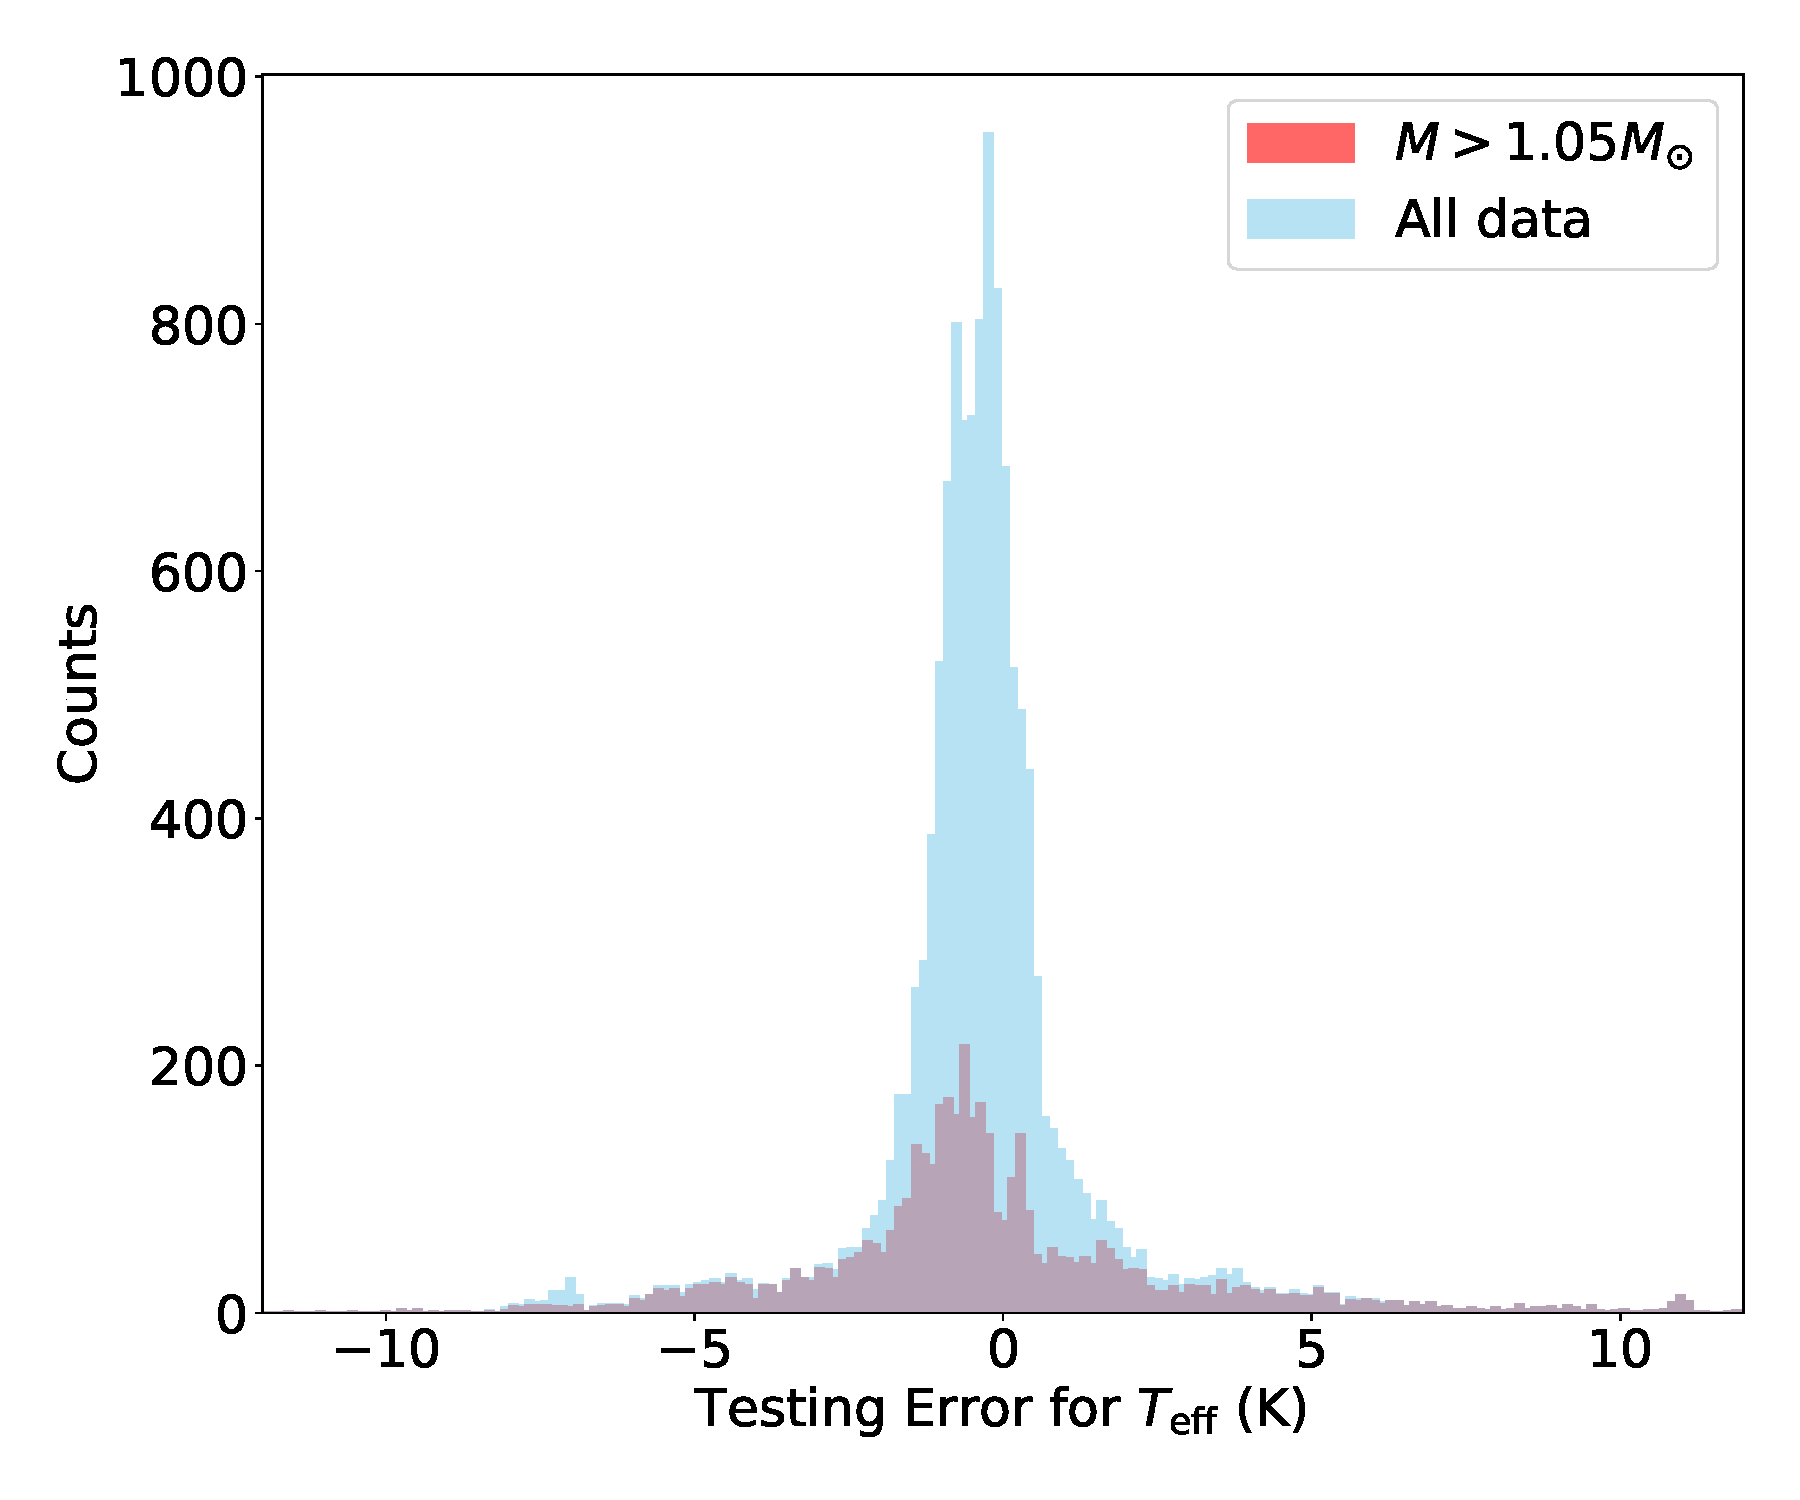
\includegraphics[width=1.0\columnwidth]{2d_testing_hist_effective_T.pdf}	
    \caption{Top: The 2D GP model for $T_{\rm eff}$. Bottom: probability distributions of validating errors of the GP model. }  
    \label{fig:2dtest}
\end{figure}

It can be seen in Figure \ref{fig:2dtest} that the kernel function in the area of $M \geq 1.05 {\rm M_{\odot}}$ and ${\it EEP} \leq 0.7$ is more complex than that for other regions. This particular area are relatively difficult to learn and poorly predicted by the GP model. 
%
There are two regions where global parameters vary relatively fast. The first is around the `hook' and main-sequence-turn-off point ({\it EEP} $\sim$ 0.4) where high-mass tracks sharply turns on the HR diagram. The second is at early subgiant pahse ({\it EEP} $\sim$ 0.6) where stars fast restructure. 
%
When there is a subregion in which the GP model performs worse than other areas, the error distribution would not follow a Normal function. As shown at the bottom of Figure \ref{fig:2dtest}, the density distribution of testing errors form long tails which contents about $10\%$ data. 
%
We inspect testing errors for other four outputs. The cases of surface gravity and radius are similar to the effective temperature. The region where the surface metallicity quickly changes is not at the hook but at the early subgiant phase in relatively high-mass tracks. This is because high-mass models maintain shallow convective envelope and hence have strong diffusion effect during the main-sequence stage. At the early subgiant phase, the quick expansion of the surface convective envelope mixes up the settled heavy elements, leading to a fast raise of the surface metallicity. 
%
We also find that the accuracy of age prediction drops down for very old low-mass stellar models. This is because age values vary in a relatively big dynamic range (15 - 50 Gyr) in a small fraction of data points. Poor GP predictions are caused by the low age resolution.         
 

The error distribution causes an issue in validating and testing GP models. In the training process, we normally use some global errors, such like Root Mean Square Error (RMSE), to represent the validation or testing results. For this case, a global error indicates the general accuracy but is not able to point out how GP performs in the regions where an observable quantity quickly varies. 
%
We hence want to have an error index that can reflect the GP model performance in those sub-areas. By inspecting the error distributions of all five outputs, we find the data points in the tails (outside the 3 times of full width at half maximum) are around 10\% (8 - 12\% for different outputs).  For the majority (90\%) of data points, which from a Gaussian-like profile, the 68\% confidential interval (1-$\sigma$ uncertainty) can be used to reflect the global accuracy. For the worst 10\% of the data, we could use the 95\% and 99.7\% confidential intervals (2- and 3-$\sigma$ uncertainties) to describe the median and the length of the tail. Thus, we define an Error Index (EI), which is the sum of 68\%, 95\%, and 99.7\% cumulative values of the absolute errors. For the case in Figure \ref{fig:2dtest}, cumulative values at 68\%, 95\%, and 99.7\% are 1.1, 4.9, and 11.1K, which give a testing EI equals to 17.1K. We apply this EI in all following training processes to validate and test GP models. 

We train GP models using different kernel functions to investigate which is the best for our application. We do this with the 2D data because the training is fast to be able to test many different options. As mentioned in Section \ref{sec:kernel}, we find Mat32 is the most suitable kernel for mapping the stellar model grid.  


\subsection{3D Problem: Strategy for Large Data Sample}\label{sec:3d}

We apply GP to a 3D problem where GP maps three fundamental inputs, i.e., mass, EEP, and metallicity to five observables. The main purpose of this preliminary study is investigate the strategy for training large data sample exceeding the data size limitation. 
%
We select training data from the primary grid with $Y_{\rm init}$ = 0.28 and $\alpha_{\rm MLT}$ = 2.1. The training dataset contents $\sim$300,000 data points which is 15 times the limit of training data size (20,000).  For validating and testing purposes, we compute another 174 evolutionary tracks with the same input $Y_{\rm init}$ and $\alpha_{\rm MLT}$ but random input $M$ and [Fe/H]$_{\rm init}$. 

We start with sampling only 20,000 training data from the 3D model grid to train GP models. We use the testing EIs of these models as standard references. For instance, the testing EI for $T_{\rm eff}$ is 23.5K (2.0, 5.8, and 15.7 K at 68th, 95th, and 99.7th). 
%
We then apply two state-of-the-art approaches designed for large dataset to train the model. These two approaches are named as Stochastic Variational GP (SVGP) and Structured Kernel Interpolation (SKI GP). We find some minor improvements in the GP predictions. Comparing the testing EI for $T_{\rm eff}$, SVGP gives a results of EI = 24.1K (2.2, 6.8, and 15.1K at  at 68th, 95th, and 99.7th) and SKI GP ends up with  EI = 22.9K (2.0, 6.1, and 14.8K at 68th, 95th, and 99.7th). Details about these two implements and some discussions about the results can be seen in appendix \ref{app:B}. However, later tests on 5D data show that these two methods can not significantly improve the GP performances, and we hence seek other methods for better training GP models.


 \begin{figure}
	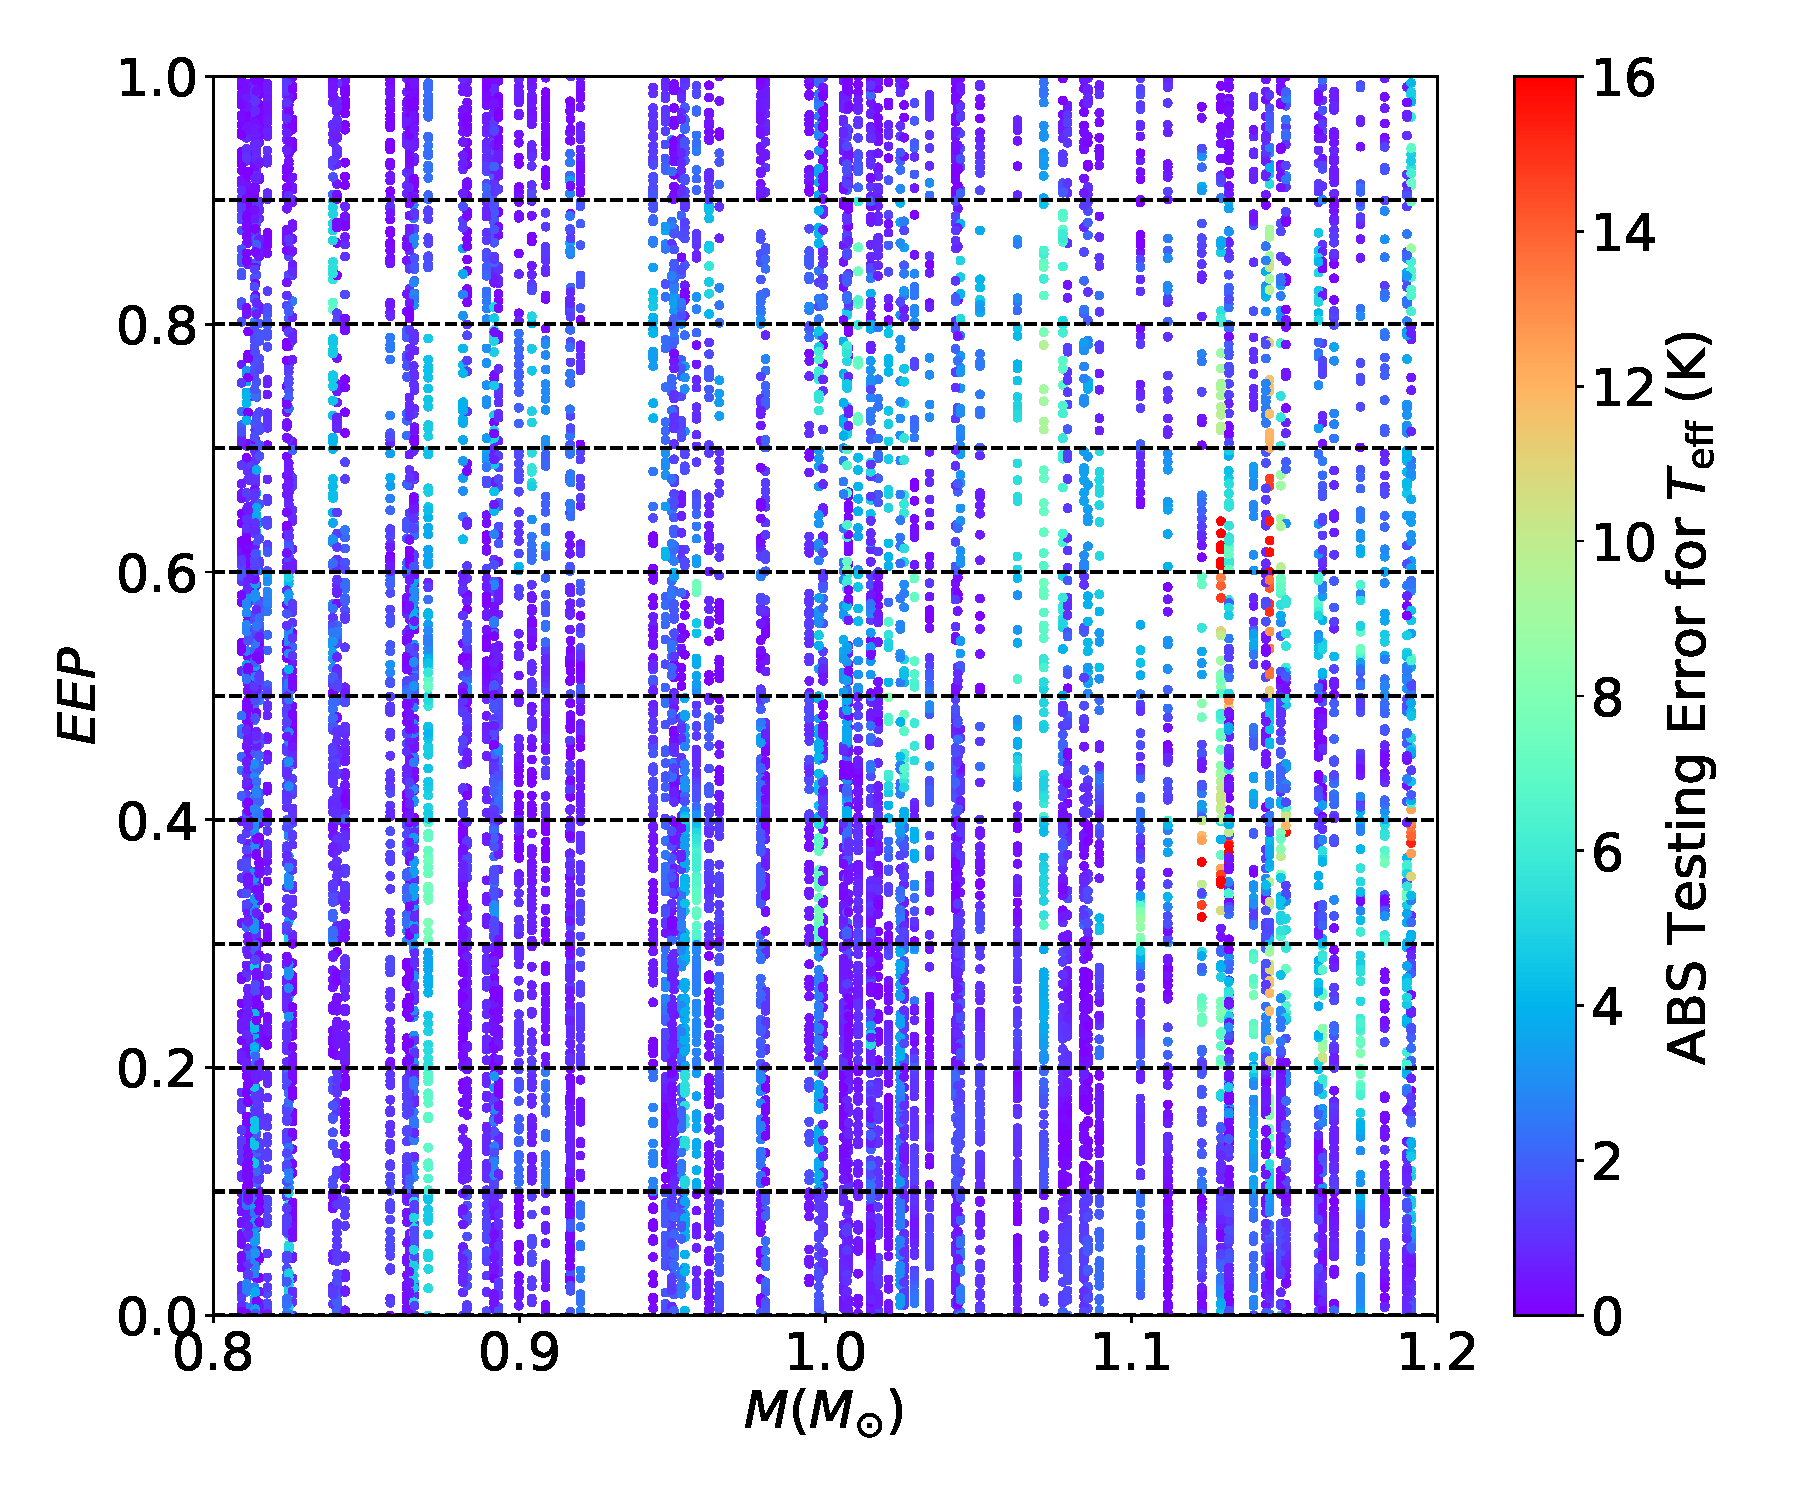
\includegraphics[width=1.0\columnwidth]{3d-testing_teff-10sections.pdf}
	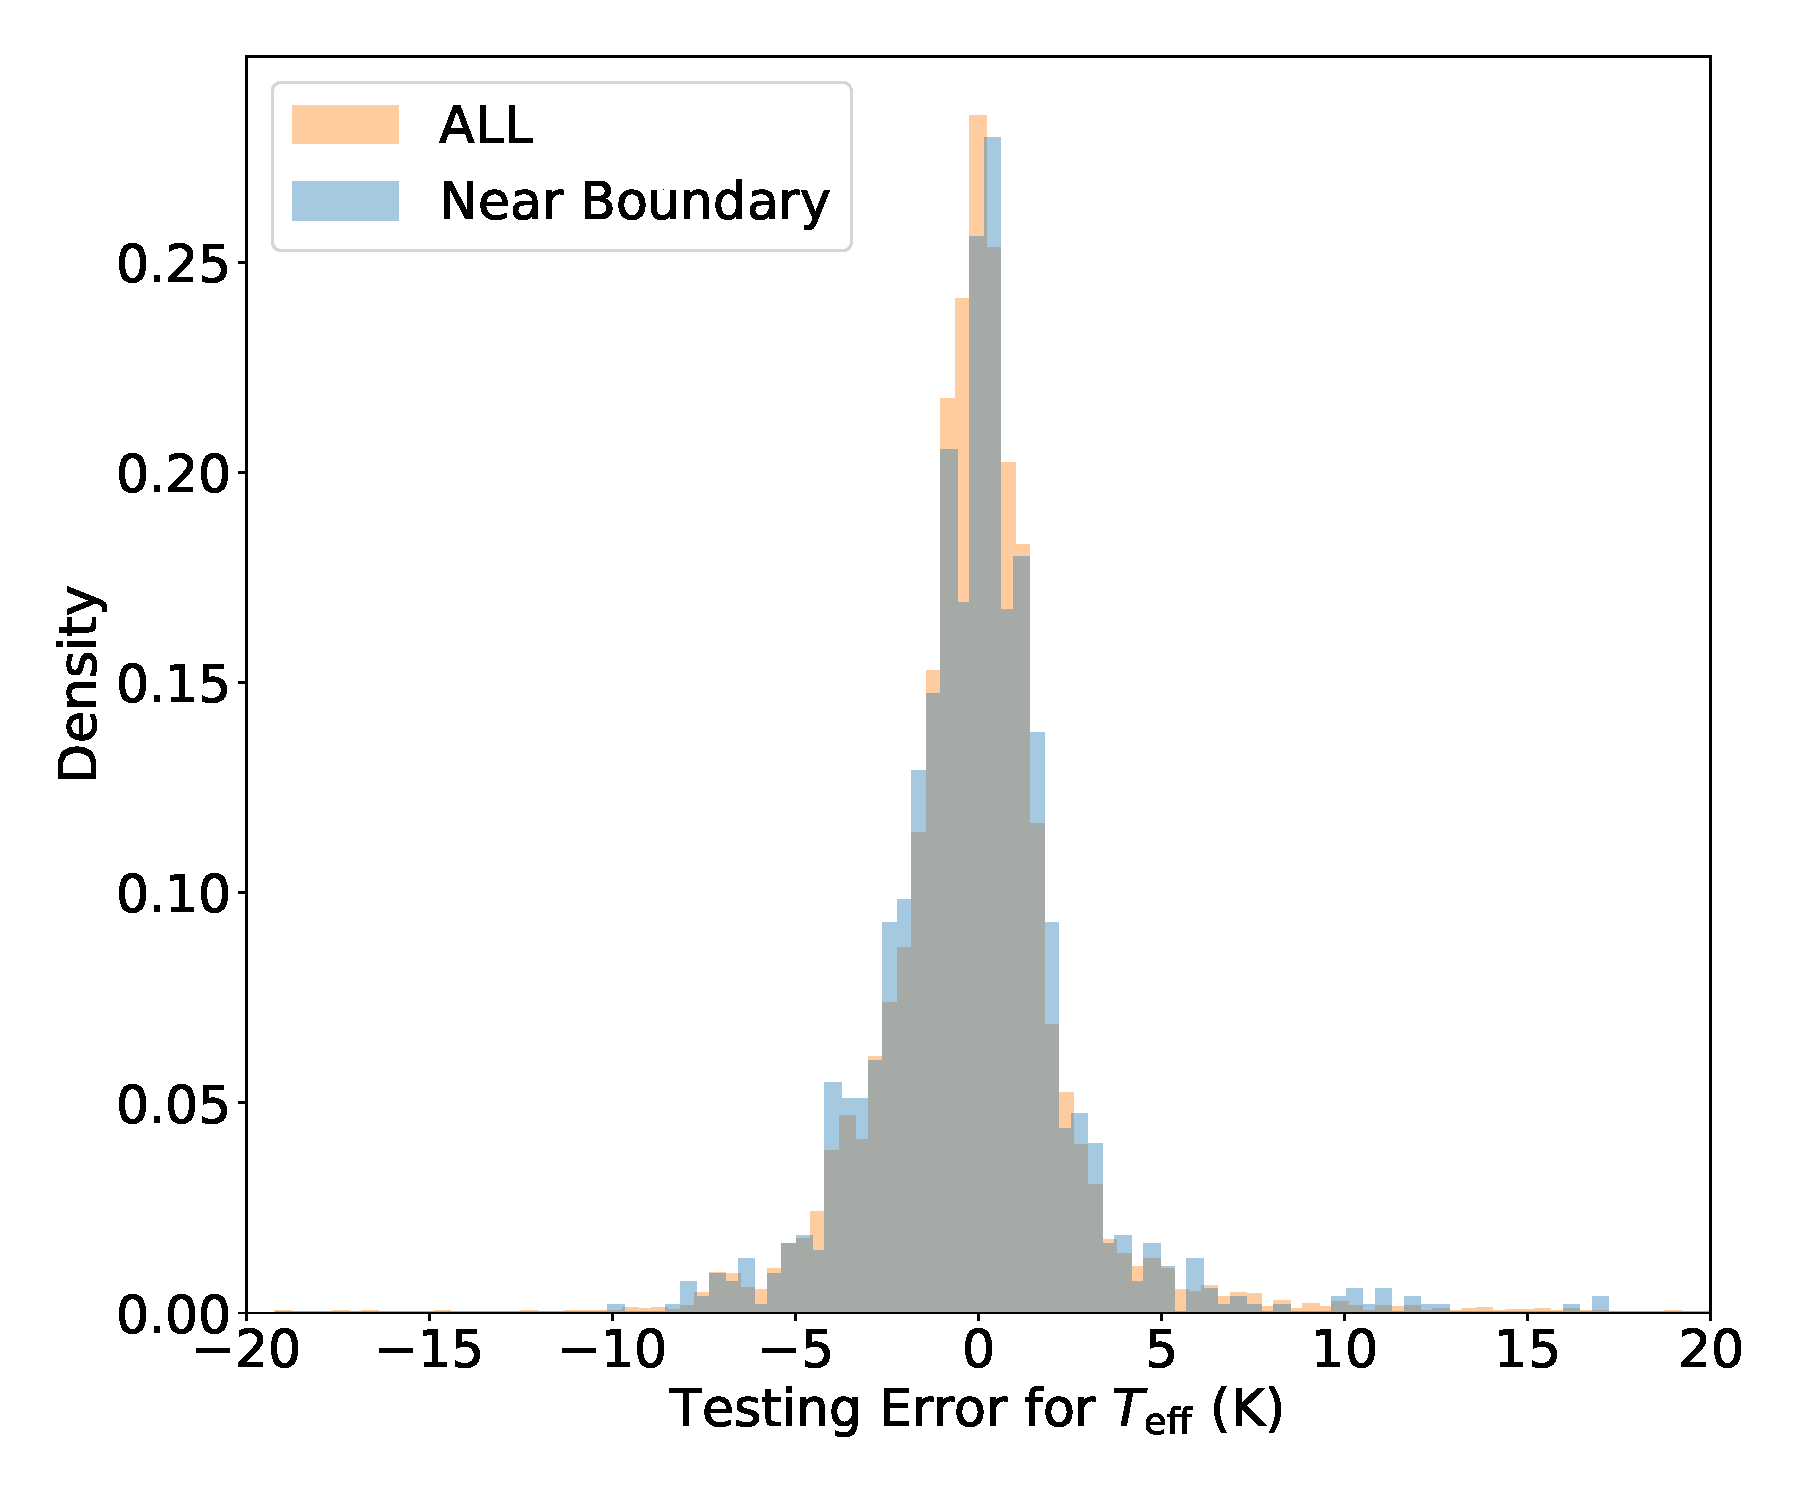
\includegraphics[width=1.0\columnwidth]{3d-testing_teff-hist-10sections.pdf}	
    \caption{Top: Testing errors of 3D GP model for $T_{\rm eff}$ on the $M - EEP$ diagram. Dashes indicates section boundaries. Bottom: examination of the edge effects of the section scenario. Probability distributions of testing errors of all testing data and those near the boundary ($\pm$0.01 EEP) in the upper graph are compared.  As it can be seen, testing errors do not raise around the boundary. }  
    \label{fig:3dtest}
\end{figure}


The GPU memory captivity limits the actual number of data that induce the kernel function. This limitation becomes critical for the high-demission applications because we need much more data give the fact that the parameter space exponentially increase with input demission. 
%
A simple way to overcome this issue is breaking the grid into many sections and train GP models for each section separately. 
We divide the training dataset into 10 equal sections by {\it EEP} and sample 20,000 training data in each. A set of GP models are then trained for each {\it EEP} section. 
%
Using this section scenario, we improve the testing EIs for the five output parameters by around 10\%. For instance, the testing EI for $T_{\rm eff}$ decreases from 23.5 to 21.6K. (1.7, 5.0, 14.9K at at  at 68th, 95th, and 99.7th). EI values for the five outputs before and after sectioning the training dataset can be seen in Table~\ref{tab:results}.  On this 3D problem, the section scenario performs slightly better than the SVGP and SKI GP, but it makes more significant improvements in training the 5D dataset, where the SVGP and SKI GP approaches become less reliable for high-demission problems. 
We hence apply this section scenario as our training strategy. 
 
The section scenario improves the performance of GP model, but there is a major concern about the edge effect at the boundary between segments. If the GP model works significantly poorly at these boundaries, it will be difficult to map the systematic errors across the whole parameter space. We hence examine potential edge effects as illustrated in Figure~\ref{fig:3dtest}. We inspect absolute testing errors for each output on the $M-EEP$ diagram. No obvious edge effect is found. We also do a statistical comparison between all errors and those around section boundaries ($\pm0.01EEP$). As shown in the bottom graph, the density distributions of the two samples are very similar to each other. We hence adopt the section scenario as our training strategy. 



